\subsection{Random Forest}\label{ssec:randomforest}
Random forest is an ensemble of Decision Trees \cite{ho1995random} which were described in Subsection \ref{ssec:decisiontree}. This technique utilizes multiple Decision Trees (weak learners) known as estimators to average out the predictions made by each tree, and this is done to reduce overfitting and to reduce the low bias, high variance trade-off found in a Decision Tree. There are many variations for the Random Forest implementation but it depends on the dataset being used. The bagging technique is usually used when the dataset has low bias and high variance. On the other hand, boosting is used when having high bias and low variance. In the end this aims to reduce certain undesirable implications found in a Decision Trees due to its properties. 

\noindent Random Forests by their default nature, use a technique called random subspace method (Feature Bagging), which essentially selects random features, and each Decision Tree in the forest is trained using these randomly selected features. What this mean is that for each Decision Tree only a percentage of the features are randomly selected to be used in the training phase of each Decision Tree. This will reduce the correlation between each Decision Tree. The number of features to be selected randomly can be computed by; using a fixed number (smaller than the total number of features), a percentage of the total amount of features or by taking the square root, or log base 2 of the total amount of features. Furthermore, this can be also applied to bag the instances in the dataset. Meaning the full dataset is not passed to each estimator, but a subset of the dataset is used instead. Bagging the dataset is done with replacement. The total number of instances to be passed to each estimator can be computed using the same techniques when finding the total amount of features to pass in the random subspace method. Again, this will further reduce correlation between each Decision Tree.  

\noindent The other method which is used is called Boosting, and there are several variations of this technique, but for the purposes of this project ADA Boost will be described. Boosting is basically a variation on Bagging and it is used when the underlying Decision Trees are not performing well as described above. In this technique a subset of the dataset is used to train the first Decision Tree and once this process is done, all the dataset is passed to the Decision Tree to validate each instance. At this point some instances will be predicted with significant error. After this the second Decision Tree will be trained and again a random subset is chosen for training but with the exception that now the instances with significant error have a higher probability to be selected (instances are weighted according to the error). Again, the second Decision Tree is validated on the whole dataset. This procedure will go on for the number of Decision Trees to be used in the Random Forest and is done sequentially. This technique is mainly used when the dataset is not complex and have fewer number of instances so underfitting may be present. 
 
\noindent In the end when using Bagging the average of all the Decision Tree’s outcome is taken if it is a regression problem, but if it is a classification problem the majority vote is taken as a final output/prediction as shown in Figure \ref{fig:random_forest_bag}. On the other hand, in boosting, the weighted summation of each Decision Tree is taken as the final prediction. 

\begin{figure}[H]
\centering
  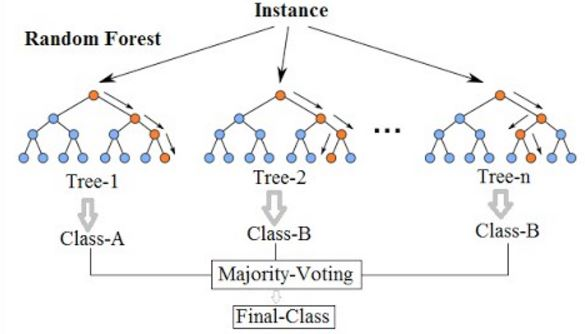
\includegraphics[scale = 0.7]{imgs/random_forest_bagging.JPG}
  \caption{Random Forest using Bagging for a classification problem}
  \label{fig:random_forest_bag}
\end{figure}

 
